\section{Discussion} \label{discussion}
\subsection{Learning curves}
As already observed in Section \ref{results}, there are clear differences between the
learning curves of the different encoder models.
To examine these differences the learning curves and their rolling standard deviation
of the \emph{train} and \emph{validation} datasets are shown on
Figure \ref{fig:learning_curves} and \ref{fig:learning_curve_stdevs} respectively.
The rolling calculation is done with a window of $10$ epochs.

Direct comparison of the models and their performances can not be done as the training
was done with the same parameter setting and no hyperparameter optimization was done.
Current remarks serve only to understand the model behavior and outline possible future
improvement options.

\begin{figure}[H]
    \centering
    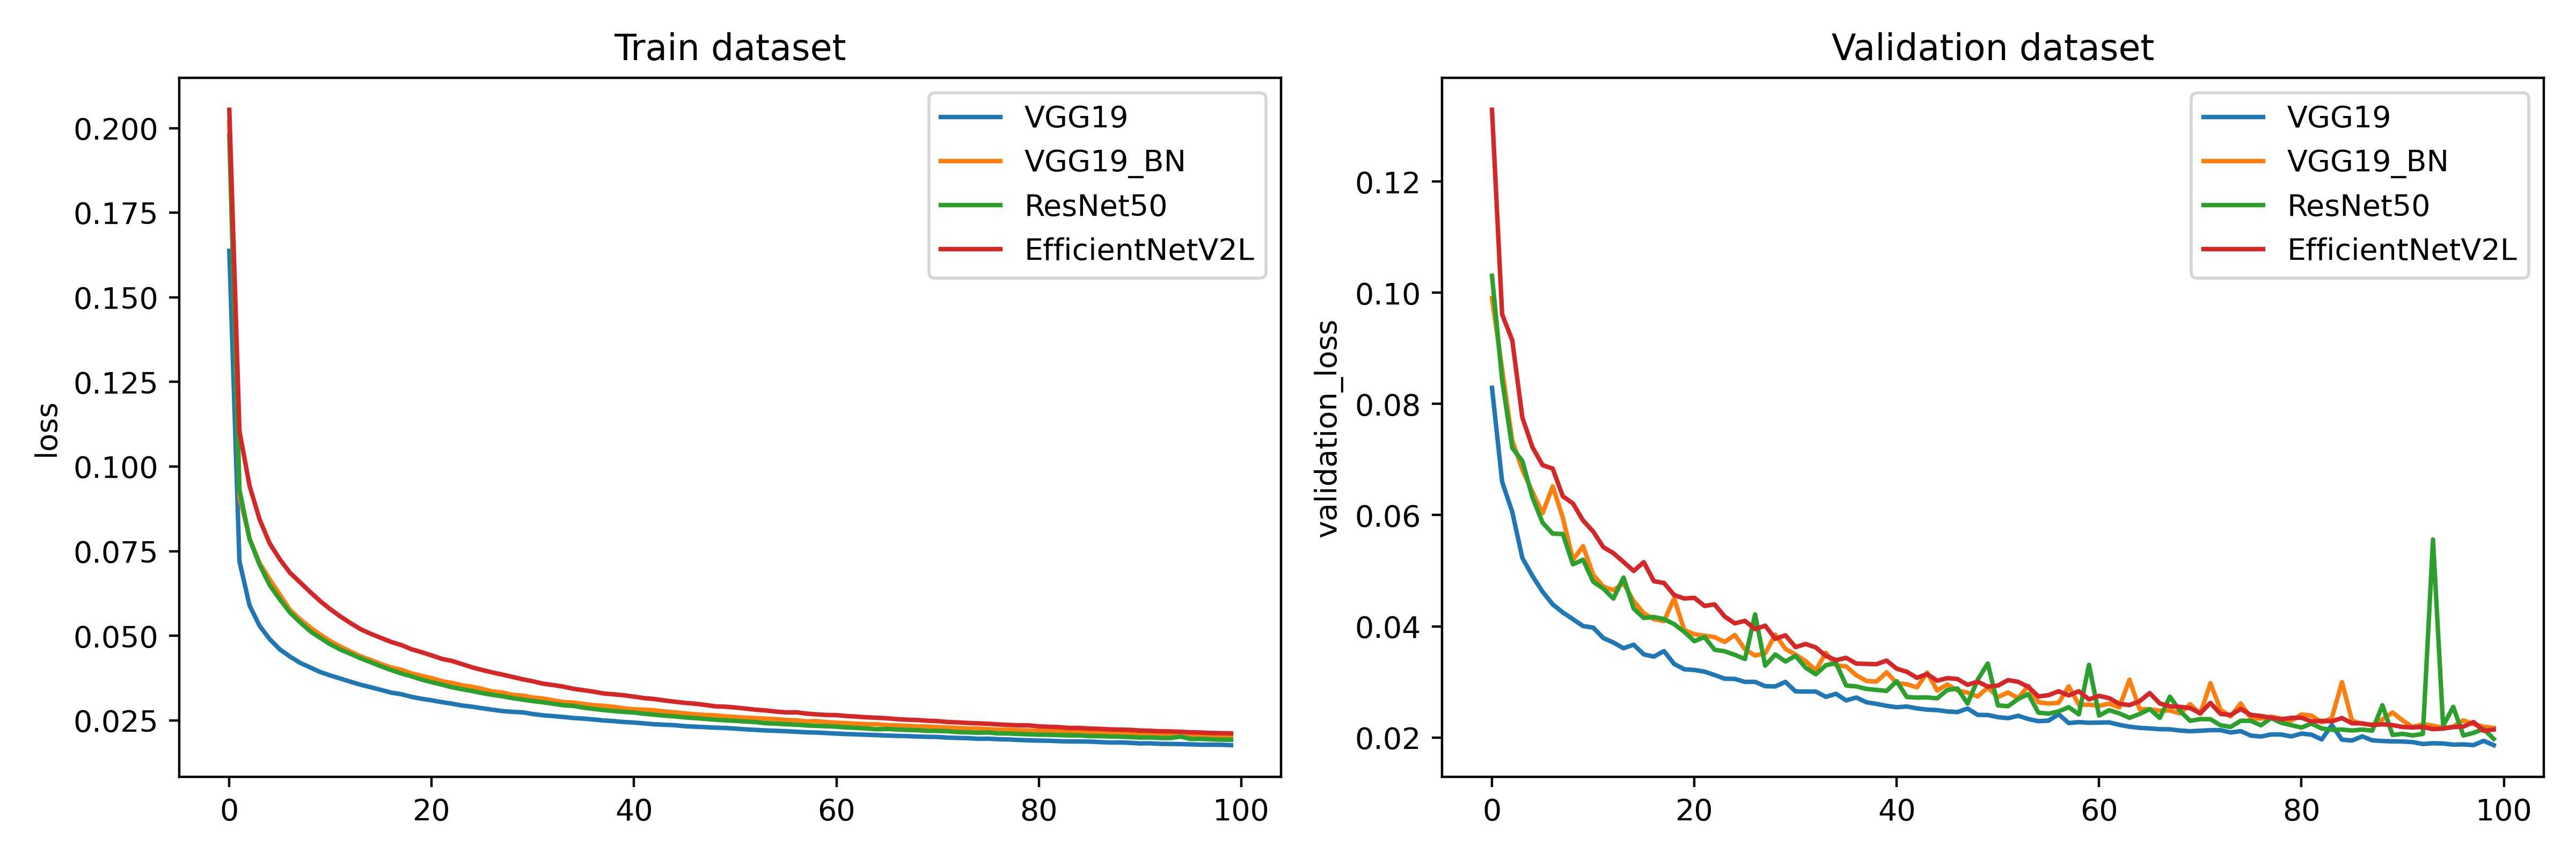
\includegraphics[width=\textwidth]{./results/comparison/learning_curves.png}
    \caption{Learning curve comparison of different encoders}
    \label{fig:learning_curves}
\end{figure}

The learning curves on the \emph{train} dataset are quite comparable, the main differences are
the starting and ending value and the gradient over the epochs.
As the starting loss heavily depend on the initialization of the starting weights, an option
would be to set these values based on a profound approach in the future.
The resulting value is quite close for each model, reaching a value around $0.02 - 0.025$.
Similar behavior is observed on the \emph{validation} dataset, the noticeable
difference is the gradient of the curve, which in this case shows a less smooth evolution.

\begin{figure}[H]
    \centering
    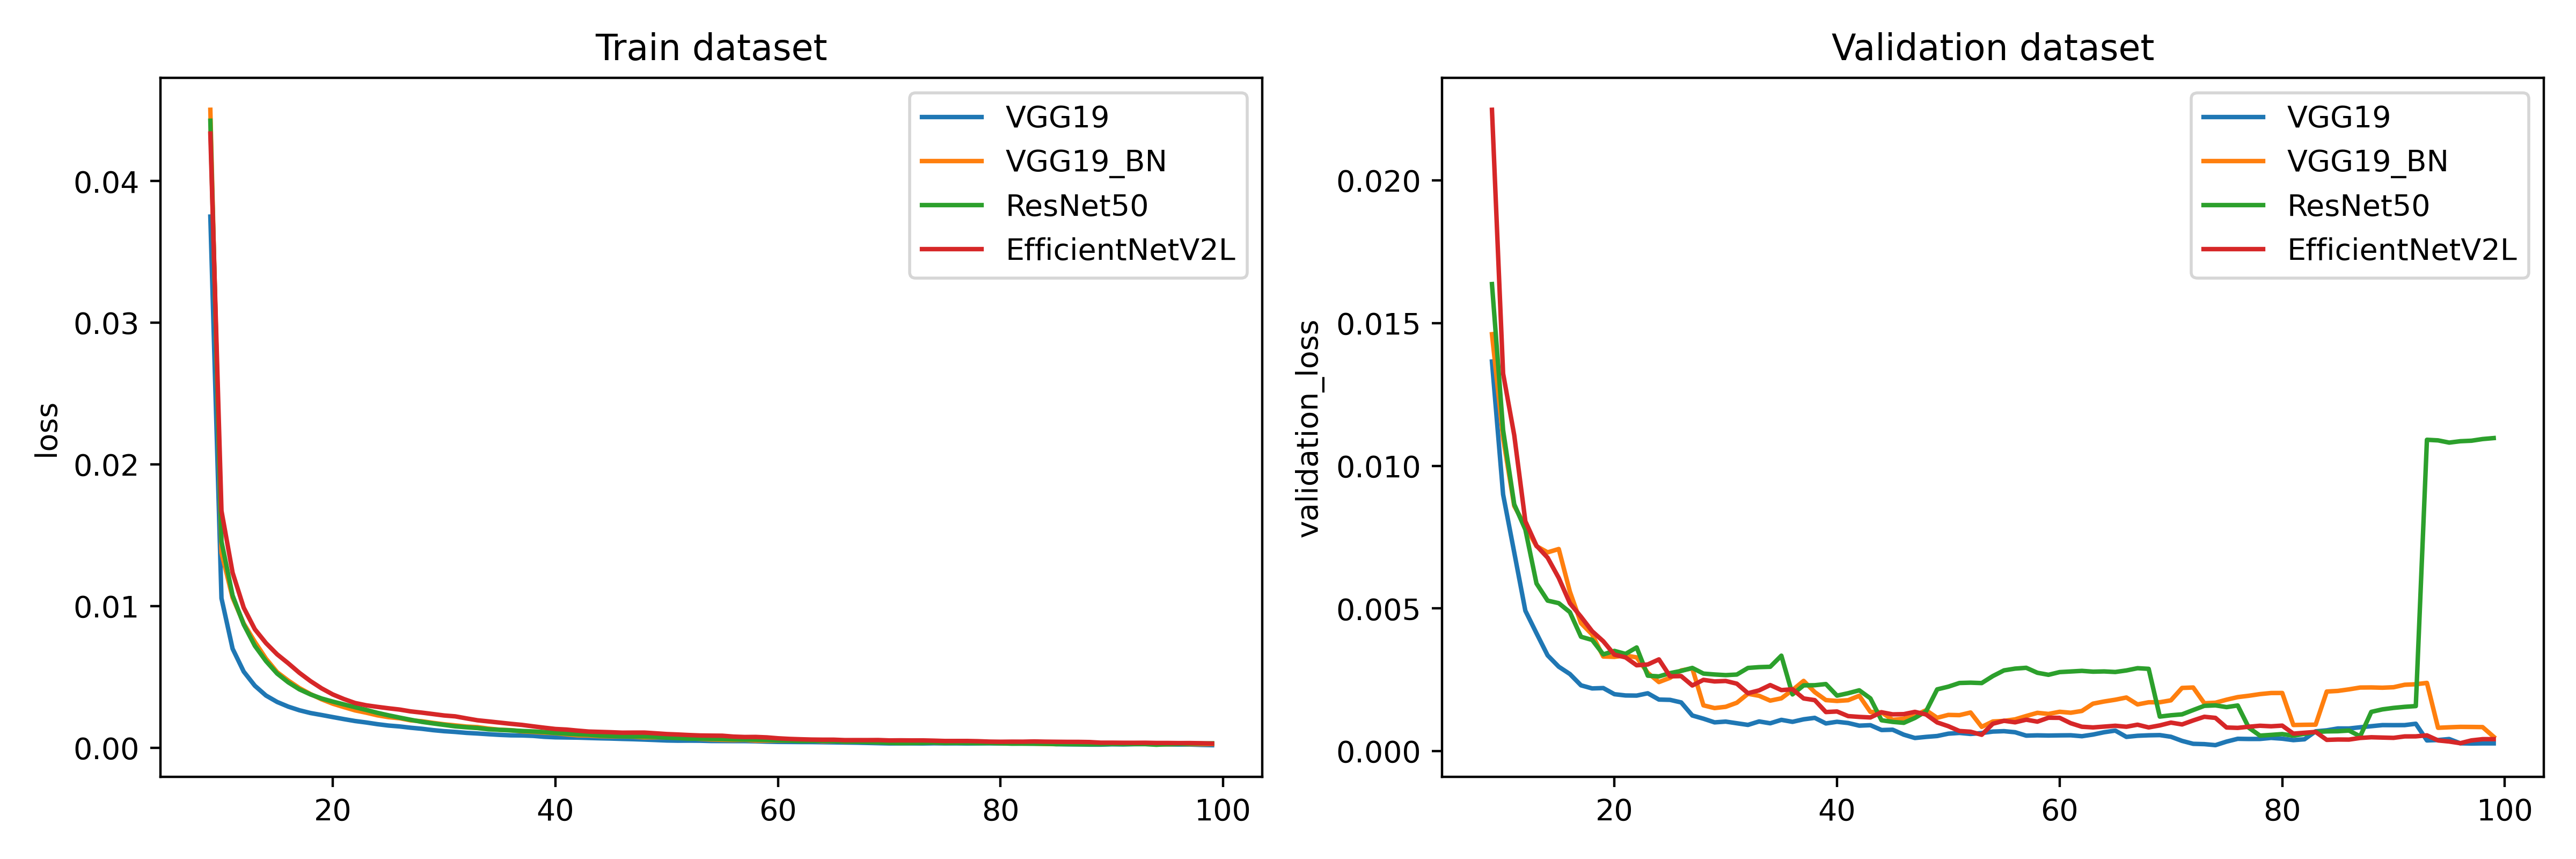
\includegraphics[width=\textwidth]{./results/comparison/stdevs.png}
    \caption{Standard deviation of learning curves}
    \label{fig:learning_curve_stdevs}
\end{figure}

The standard deviation of the learning curves also indicate key characteristics.
In case of the \emph{train} dataset the variation over the epochs drop rapidly
and converges towards zero.
The question can be risen whether further training would improve the model
as most of the autoencoded images are incomplete.
It might happen that the models are not complex enough to learn all the characteristics
of the images, on the other hand it could also happen that the changes of the weights,
due to their high number, average out the changes, so the optimizer can further tune
the model, but this can not be seen on the loss values clearly.
This raises the importance of introducing further monitoring measures
or different loss definitions.

The curves of the \emph{validation} dataset confirm our observations that there is a clear
difference of the variance.
The most stable is the VGG19 model, whilst the largest range is obtained by the ResNet50 model.
With adaptation of the learning rate this could be further optimized.

\subsection{Planar visualization}
The PCA combined with t-SNE resulted in a visualization that is able to trace the changing of
the images as passing through the model.
Normally all input phase representation should be the same (as we are visualizing the same
unprocessed data), however due to the stochastic nature of the t-SNE there are slight deviation
among the different representations provided.

Independently of this similar structure is grabbed on the input data forming three major clusters
of the \emph{normal} images and the outliers are embedded in all cases at the same location.
Afterwards encoding the same behavior is observed with some differences in the details.
First the outliers started to move out and separate out from the main clusters at the top right
and bottom left part.
At the bottom left part the separation was quite successful, on the top right part the models behaved
differently, the more complex models resulted in better performance.
The VGG19 retained these top right outliers still in the main cluster, whilst the EfficientNetV2L
has remarkably opened up the cluster and moved these images almost to the outside of the \emph{normal}
cluster.
Even the three major \emph{normal} clusters were separated better, and further internal structure is
suggested.

The matching of the number of filters via the additional convolutional layers did not introduce any
significant change to the planar visualization.
However, use of these layers are not mandatory and shall be investigated at a later step.

The decoding capability of the models are very impressive, the reduced dimensions are reverted
almost to the original representation that was seen during input phase.
This indicates that the Autoencoder model realizes its main function.

One further exploration was done using this visualization, that is, investigating whether the sequence
of the images can be captured on this feature plane.
This is shown on Figure \ref{fig:efficientnetv2l_pca2},
that colors the markers in the sequence as it can be seen in the video footage.
The visualization in this case was done using the EfficientNetV2L model.

\begin{figure}[H]
    \centering
    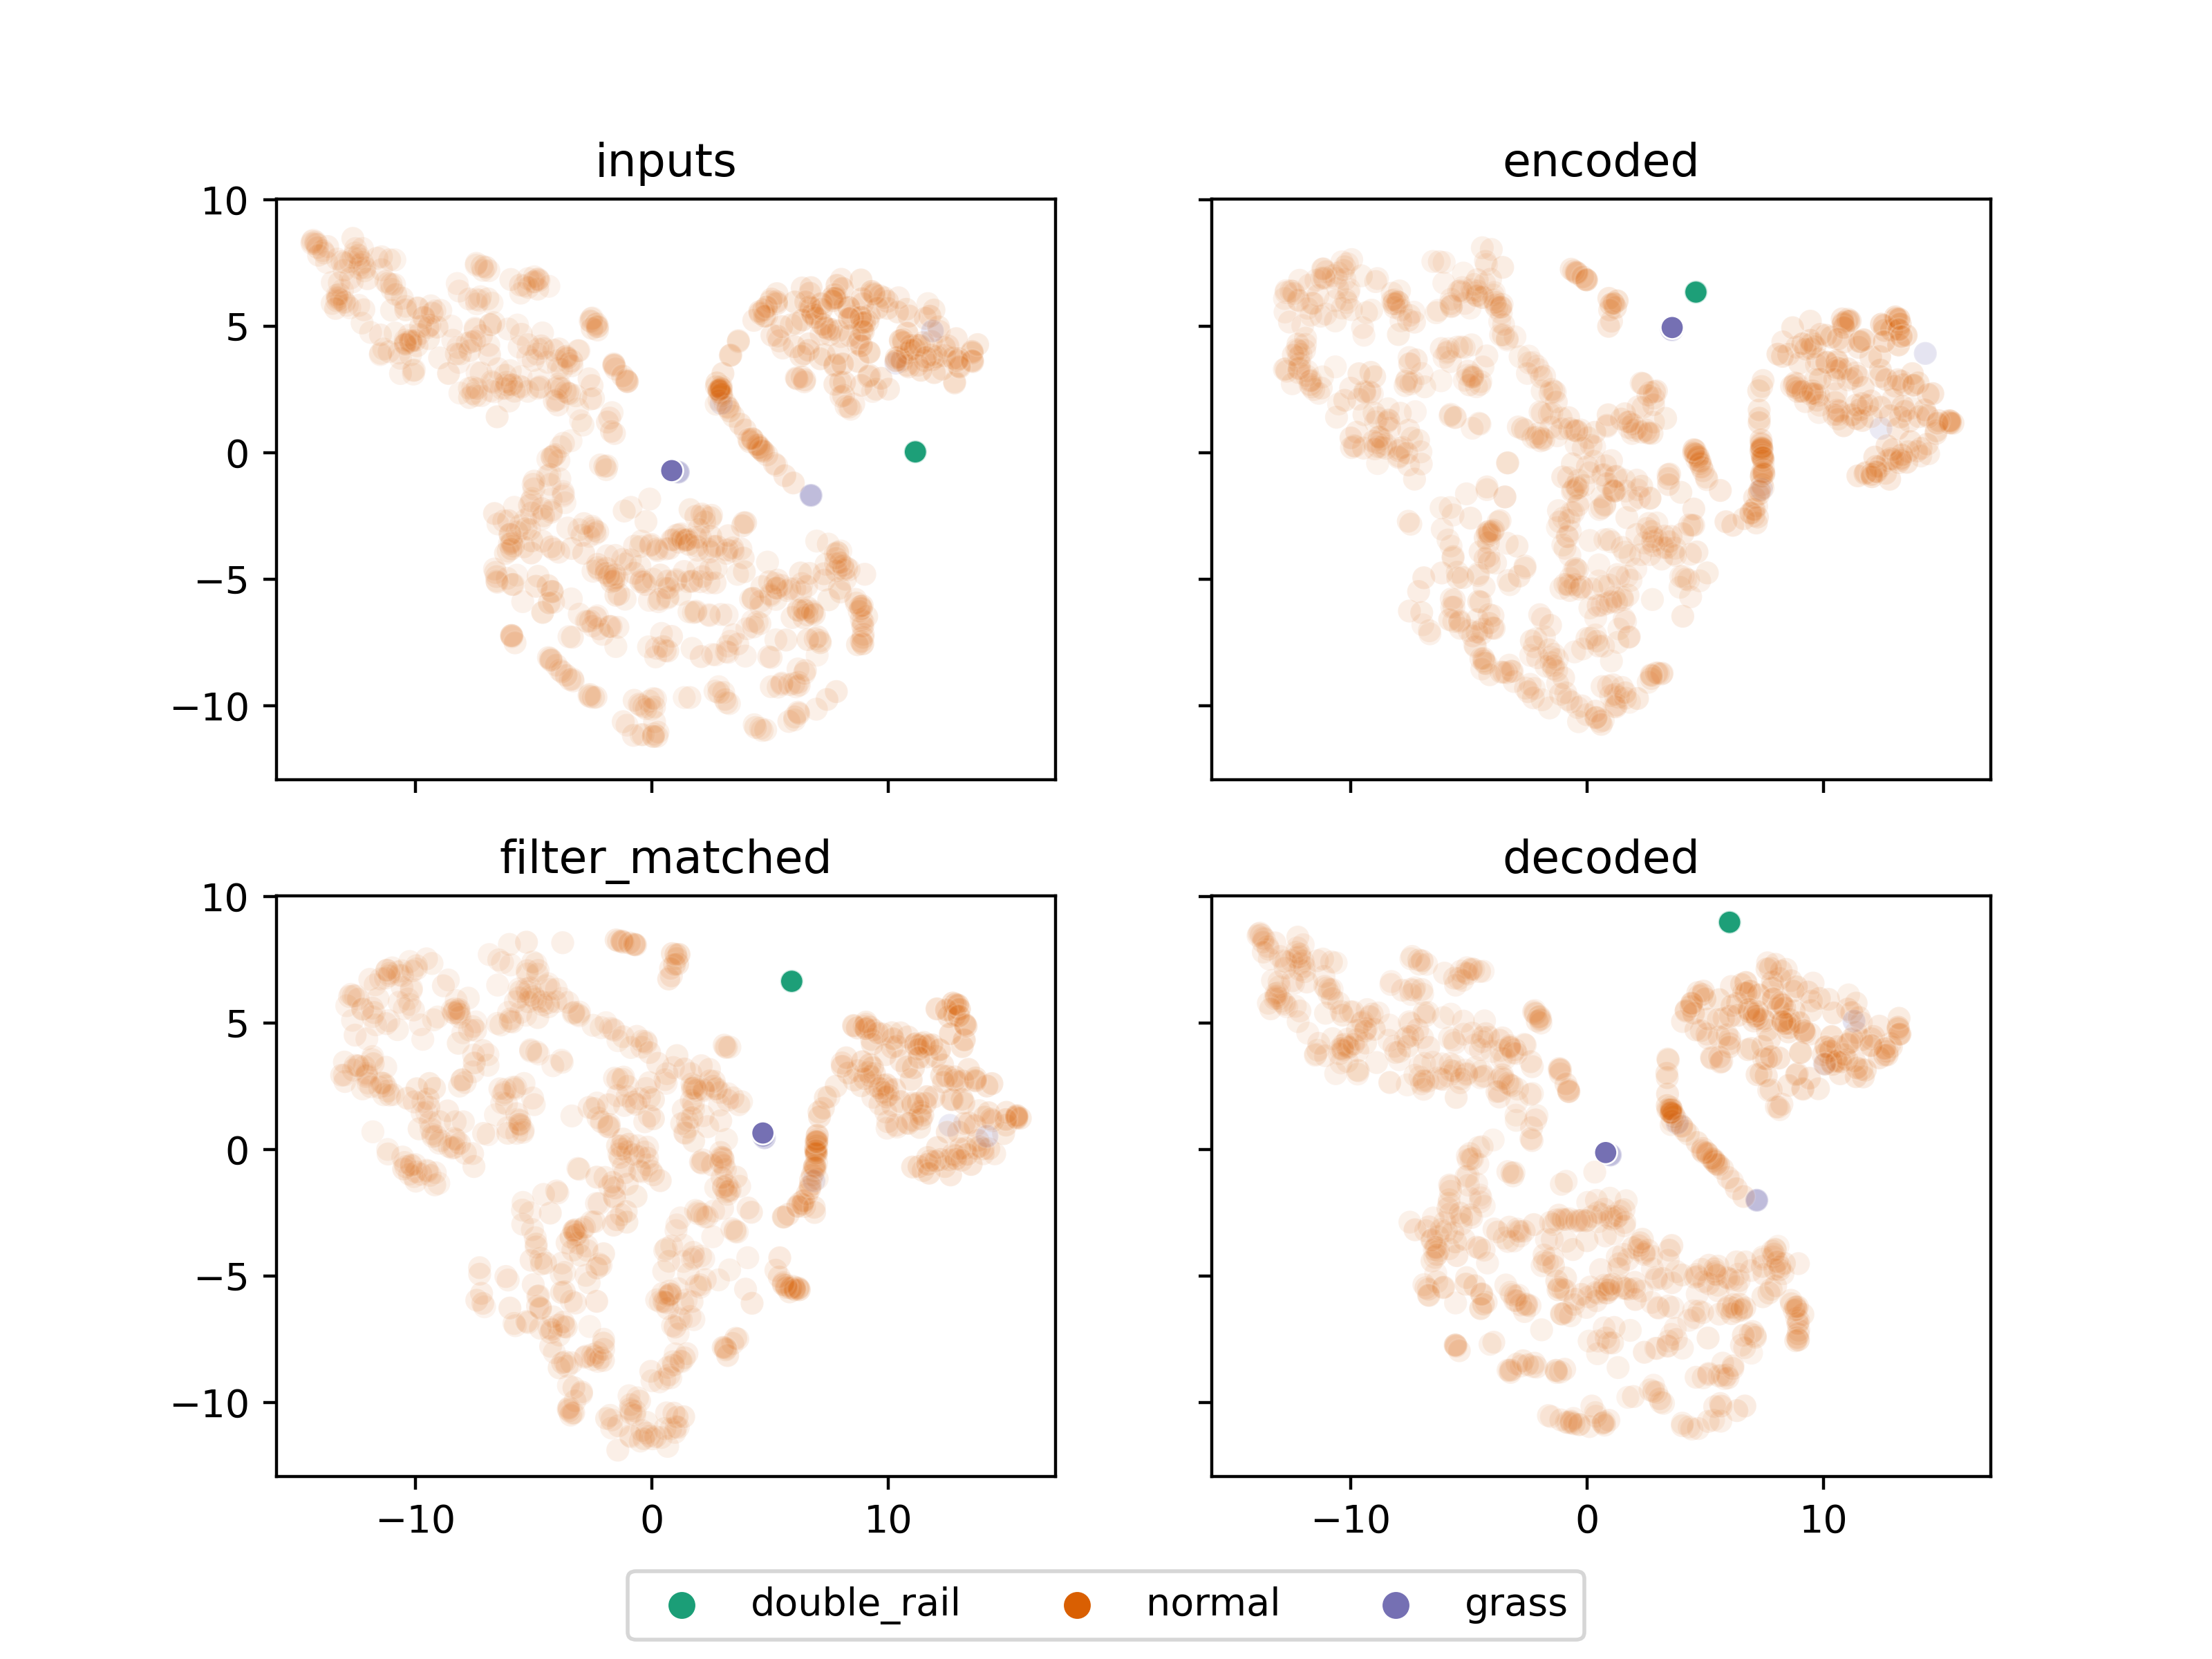
\includegraphics[width=0.8\textwidth,trim={0 1cm 0 1cm},clip]{./results/efficientnetv2l_vgg19/20230525_194238_feature_vectors_2.png}
    \caption{PCA / t-SNE representation of the sequence of the video images}
    \label{fig:efficientnetv2l_pca2}
\end{figure}

\subsection{Classification metrics}
The confusion matrices are summarized in Table \ref{table:confusion_matrices}.
This already shows that the performance of the loss-based anomaly detector is very stable,
but as stated before this happens due to the selection of the threshold value.
The Isolation Forest results highly depend on the structure of the model and resulting feature vectors.
The calculated classification metrics are shown in Table \ref{table:classification_metrics},
where LB refers to loss-based and IF refers to Isolation Forest method.

\begin{table}[H]
    \centering
    \begin{tabular}{l c |c c| c c}
        Encoder type    & True values & \multicolumn{2}{c|}{Loss-based}  & \multicolumn{2}{c}{Isolation Forest}                \\
        \hline
        VGG19           & Positive    & 31                               & 62                                   & 45    & 48   \\
                        & Negative    & 8640                             & 0                                    & 8578  & 62   \\
        \hline
        VGG19 BN        & Positive    & 30                               & 63                                   & 41    & 52   \\
                        & Negative    & 8640                             & 0                                    & 8626  & 14   \\
        \hline
        ResNet50        & Positive    & 30                               & 63                                   & 37    & 56   \\
                        & Negative    & 8640                             & 0                                    & 8577  & 63   \\
        \hline
        EfficientNetV2L & Positive    & 30                               & 63                                   & 37    & 56   \\
                        & Negative    & 8640                             & 0                                    & 8510  & 130  \\
        \hline
                        &             & False                            & True                                 & False & True \\
                        &             & \multicolumn{2}{c|}{Predictions} & \multicolumn{2}{c}{Predictions}                     \\
    \end{tabular}
    \caption{Confusion matrices of different encoders}
    \label{table:confusion_matrices}
\end{table}

The most important metrics in the actual use case is the \emph{Recall}, as it measures the proportion of outliers
found by the algorithm.
In this metric the loss-based approaches perform better than the Isolation Forest methods.
The \emph{Specificity} measures the proportion of negative hits, that is the \emph{normal} rail
in this case.
As expected, due to the heavily imbalanced dataset, this is always close to $100\%$.
The \emph{Precision} measures if there is a positive prediction what is the probability
that it really is.
Due to the threshold setting this is always maximal in case of the loss-based approaches.
The two general metrics \emph{F1 score} and \emph{Balanced accuracy} indicates the overall
performance of the models.
The first metric do not consider true negative values, therefore in our case it is more sensitive
to the performance shown on the positive predictions and true positive.
The latter one balances between true positives and true negatives.
To judge the overall performance the \emph{F1 score} and the \emph{Recall} shall be considered
simultaneously.
Not finding a true positive might increase transportation risks arising from bad track condition,
however providing too much false positives increases the cost of the maintenance (at least control
monitoring) that needs to be done, therefore due to economic reasons shall be reduced.

Based on the selected metrics the best performance is reached by the loss-based approaches,
however still not reaching an acceptable rate of \emph{Recall}.

\begin{table}[H]
    \centering
    \begin{tabular}{l | c c | c c | c c | c c}
                        & \multicolumn{2}{c|}{VGG19} & \multicolumn{2}{c|}{VGG19 BN} & \multicolumn{2}{c|}{ResNet50} & \multicolumn{2}{c}{EfficientNetV2L}                                           \\
        Metrics         & LB                         & IF                            & LB                            & IF                                  & LB       & IF      & LB       & IF      \\
        \hline
        Positives       & 93                         & 93                            & 93                            & 93                                  & 93       & 93      & 93       & 93      \\
        Negatives       & 8640                       & 8640                          & 8640                          & 8640                                & 8640     & 8640    & 8640     & 8640    \\
        True positives  & 62                         & 48                            & 63                            & 52                                  & 63       & 56      & 63       & 56      \\
        True negatives  & 8640                       & 8578                          & 8640                          & 8626                                & 8640     & 8577    & 8640     & 8510    \\
        False positives & 0                          & 62                            & 0                             & 14                                  & 0        & 63      & 0        & 130     \\
        False negatives & 31                         & 45                            & 30                            & 41                                  & 30       & 37      & 30       & 37      \\
        \hline
        Recall (Sens.)  & 66.67\%                    & 51.61\%                       & 67.74\%                       & 55.91\%                             & 67.74\%  & 60.22\% & 67.74\%  & 60.22\% \\
        Specificity     & 100.00\%                   & 99.28\%                       & 100.00\%                      & 99.84\%                             & 100.00\% & 99.27\% & 100.00\% & 98.50\% \\
        Precision       & 100.00\%                   & 43.64\%                       & 100.00\%                      & 78.79\%                             & 100.00\% & 47.06\% & 100.00\% & 30.11\% \\
        \hline
        F1 score        & 80.00\%                    & 47.29\%                       & 80.77\%                       & 65.41\%                             & 80.77\%  & 52.83\% & 80.77\%  & 40.14\% \\
        Balanced acc.   & 83.33\%                    & 75.45\%                       & 83.87\%                       & 77.88\%                             & 83.87\%  & 79.74\% & 83.87\%  & 79.36\% \\
    \end{tabular}
    \caption{Classification metrics of different encoders}
    \label{table:classification_metrics}
\end{table}

These results indicate that the fine-tuning of the loss threshold might improve the performance
of the anomaly detector models.
A simulation of the threshold value is shown on Figure \ref{fig:threshold_simulation}.
The threshold is defined as the multiplication of the standard deviation of the losses of the images.
The limit value is the loss mean and the multiplied standard deviation added.
Above this value the image is considered as outlier.
The optimum in terms of \emph{F1 score} is between $2.07$ and $2.24$ times the standard deviation added
to the mean of losses.
Such optimum gives a balance between precision and recall, indicating how well the anomalies found,
quantifying how much is found considering the false negative hits.
Further optimization possibilities, more decent modeling, more refined loss calculation is possible
to enhance the performance of the models.

\begin{figure}[H]
    \centering
    \begin{subfigure}{0.48\textwidth}
        \centering
        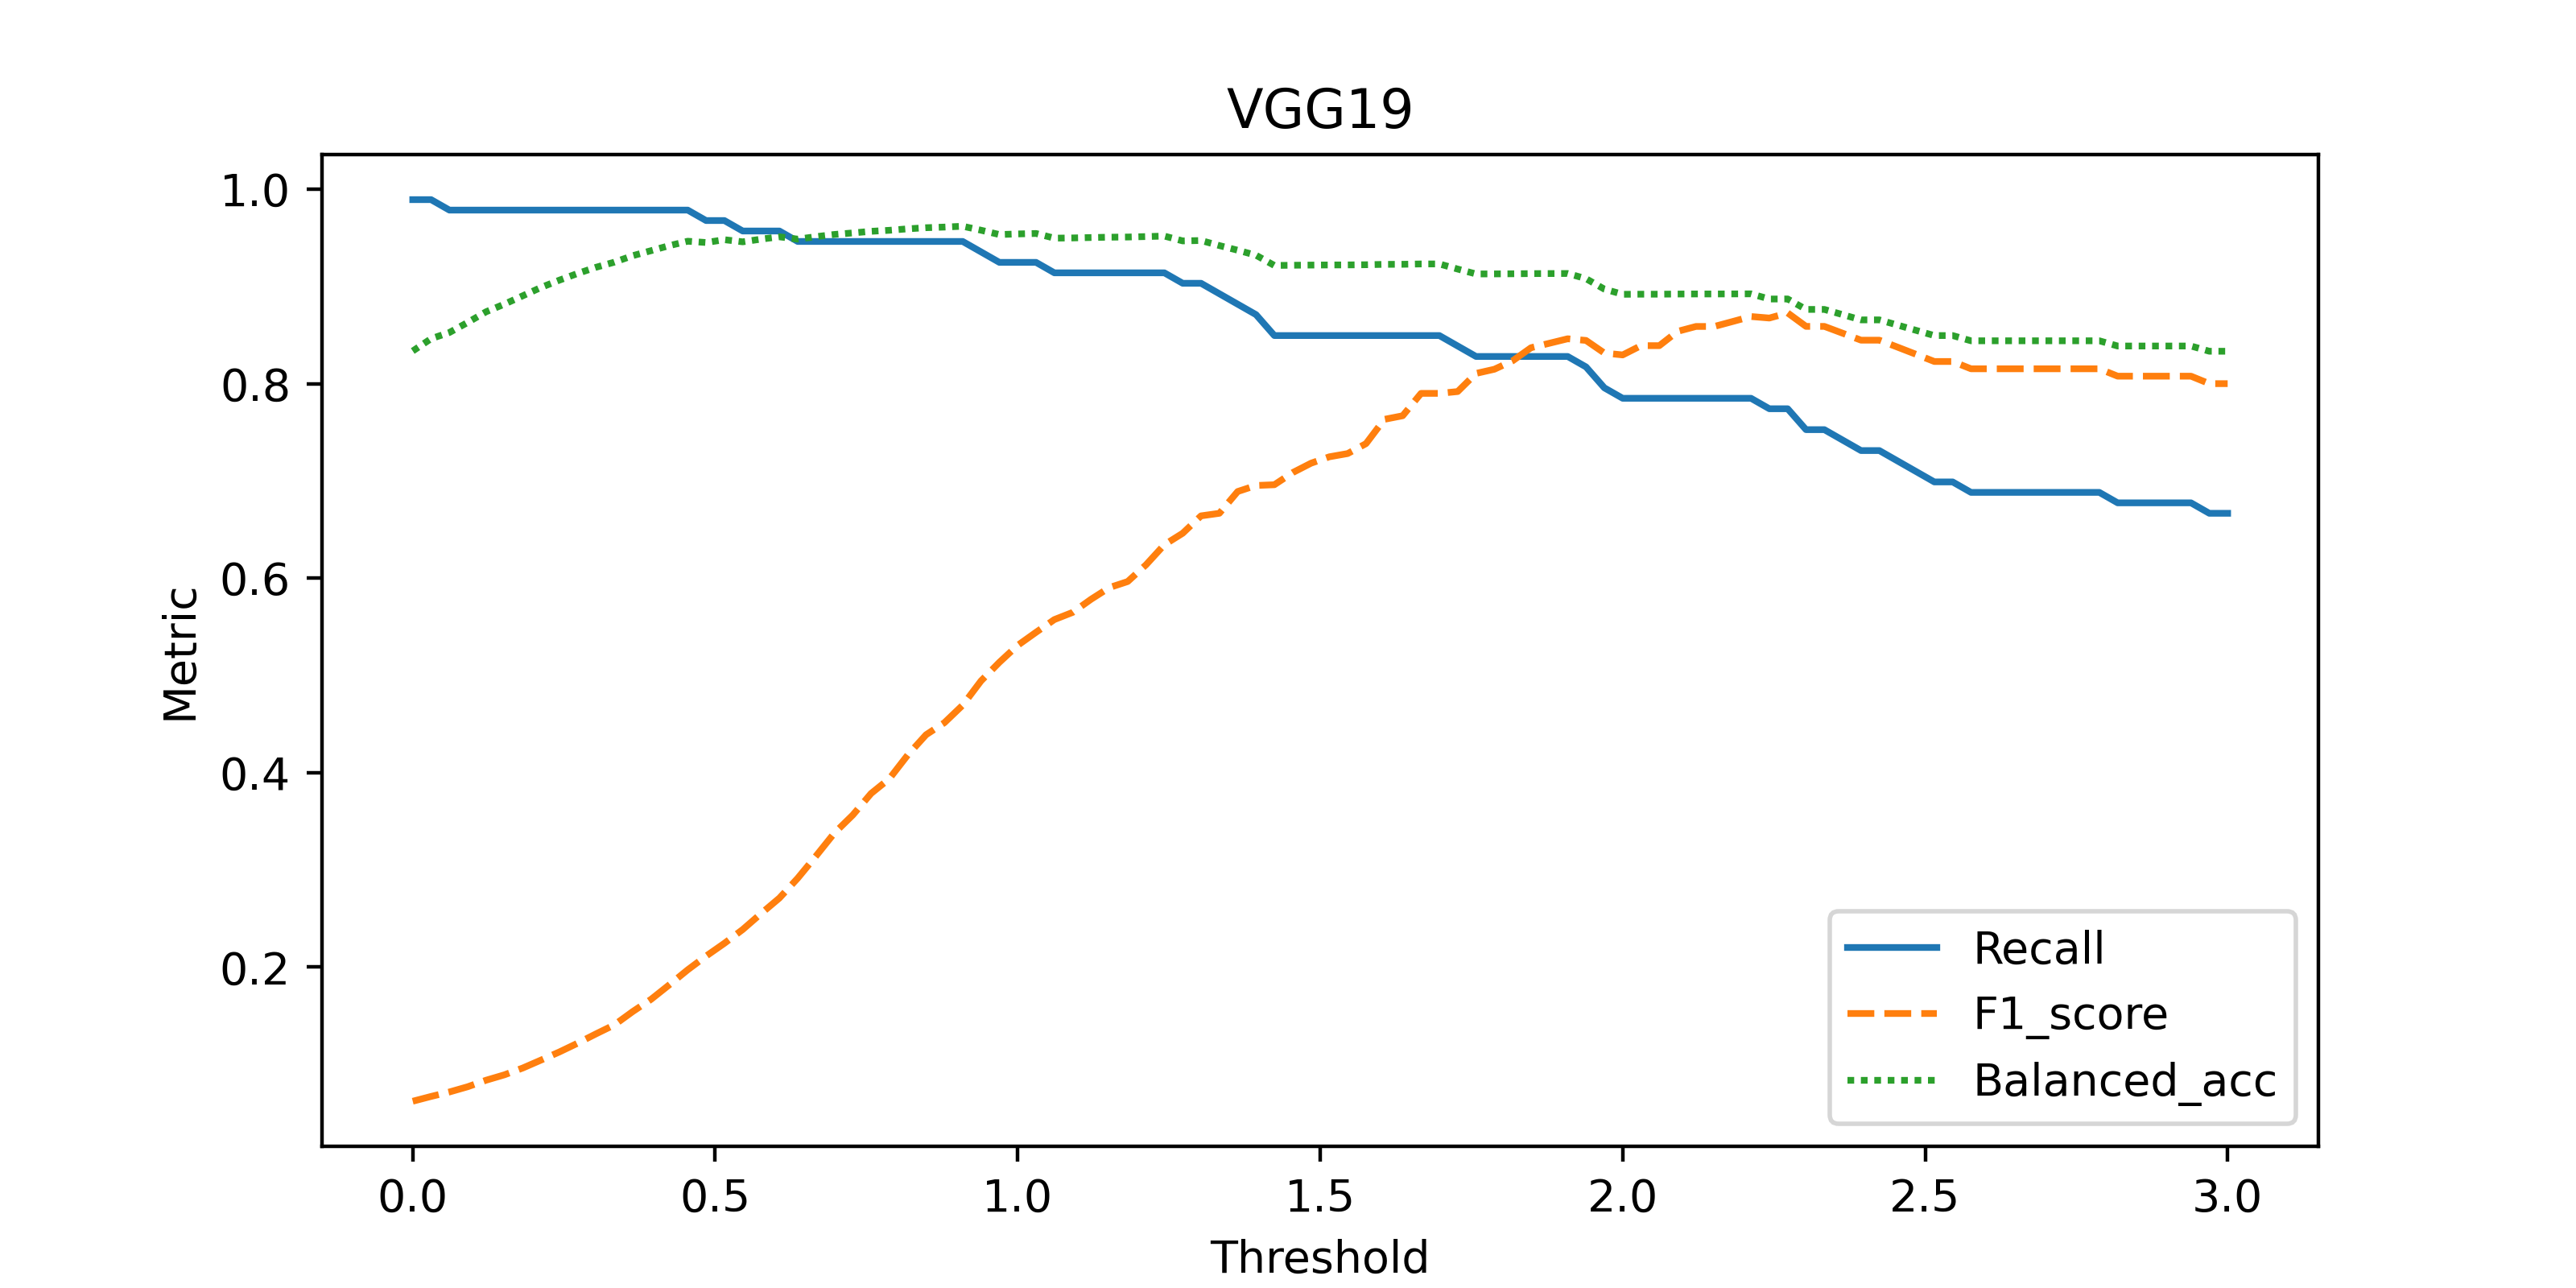
\includegraphics[width=\textwidth]{./results/comparison/VGG19_threshold.png}
    \end{subfigure}
    \begin{subfigure}{0.48\textwidth}
        \centering
        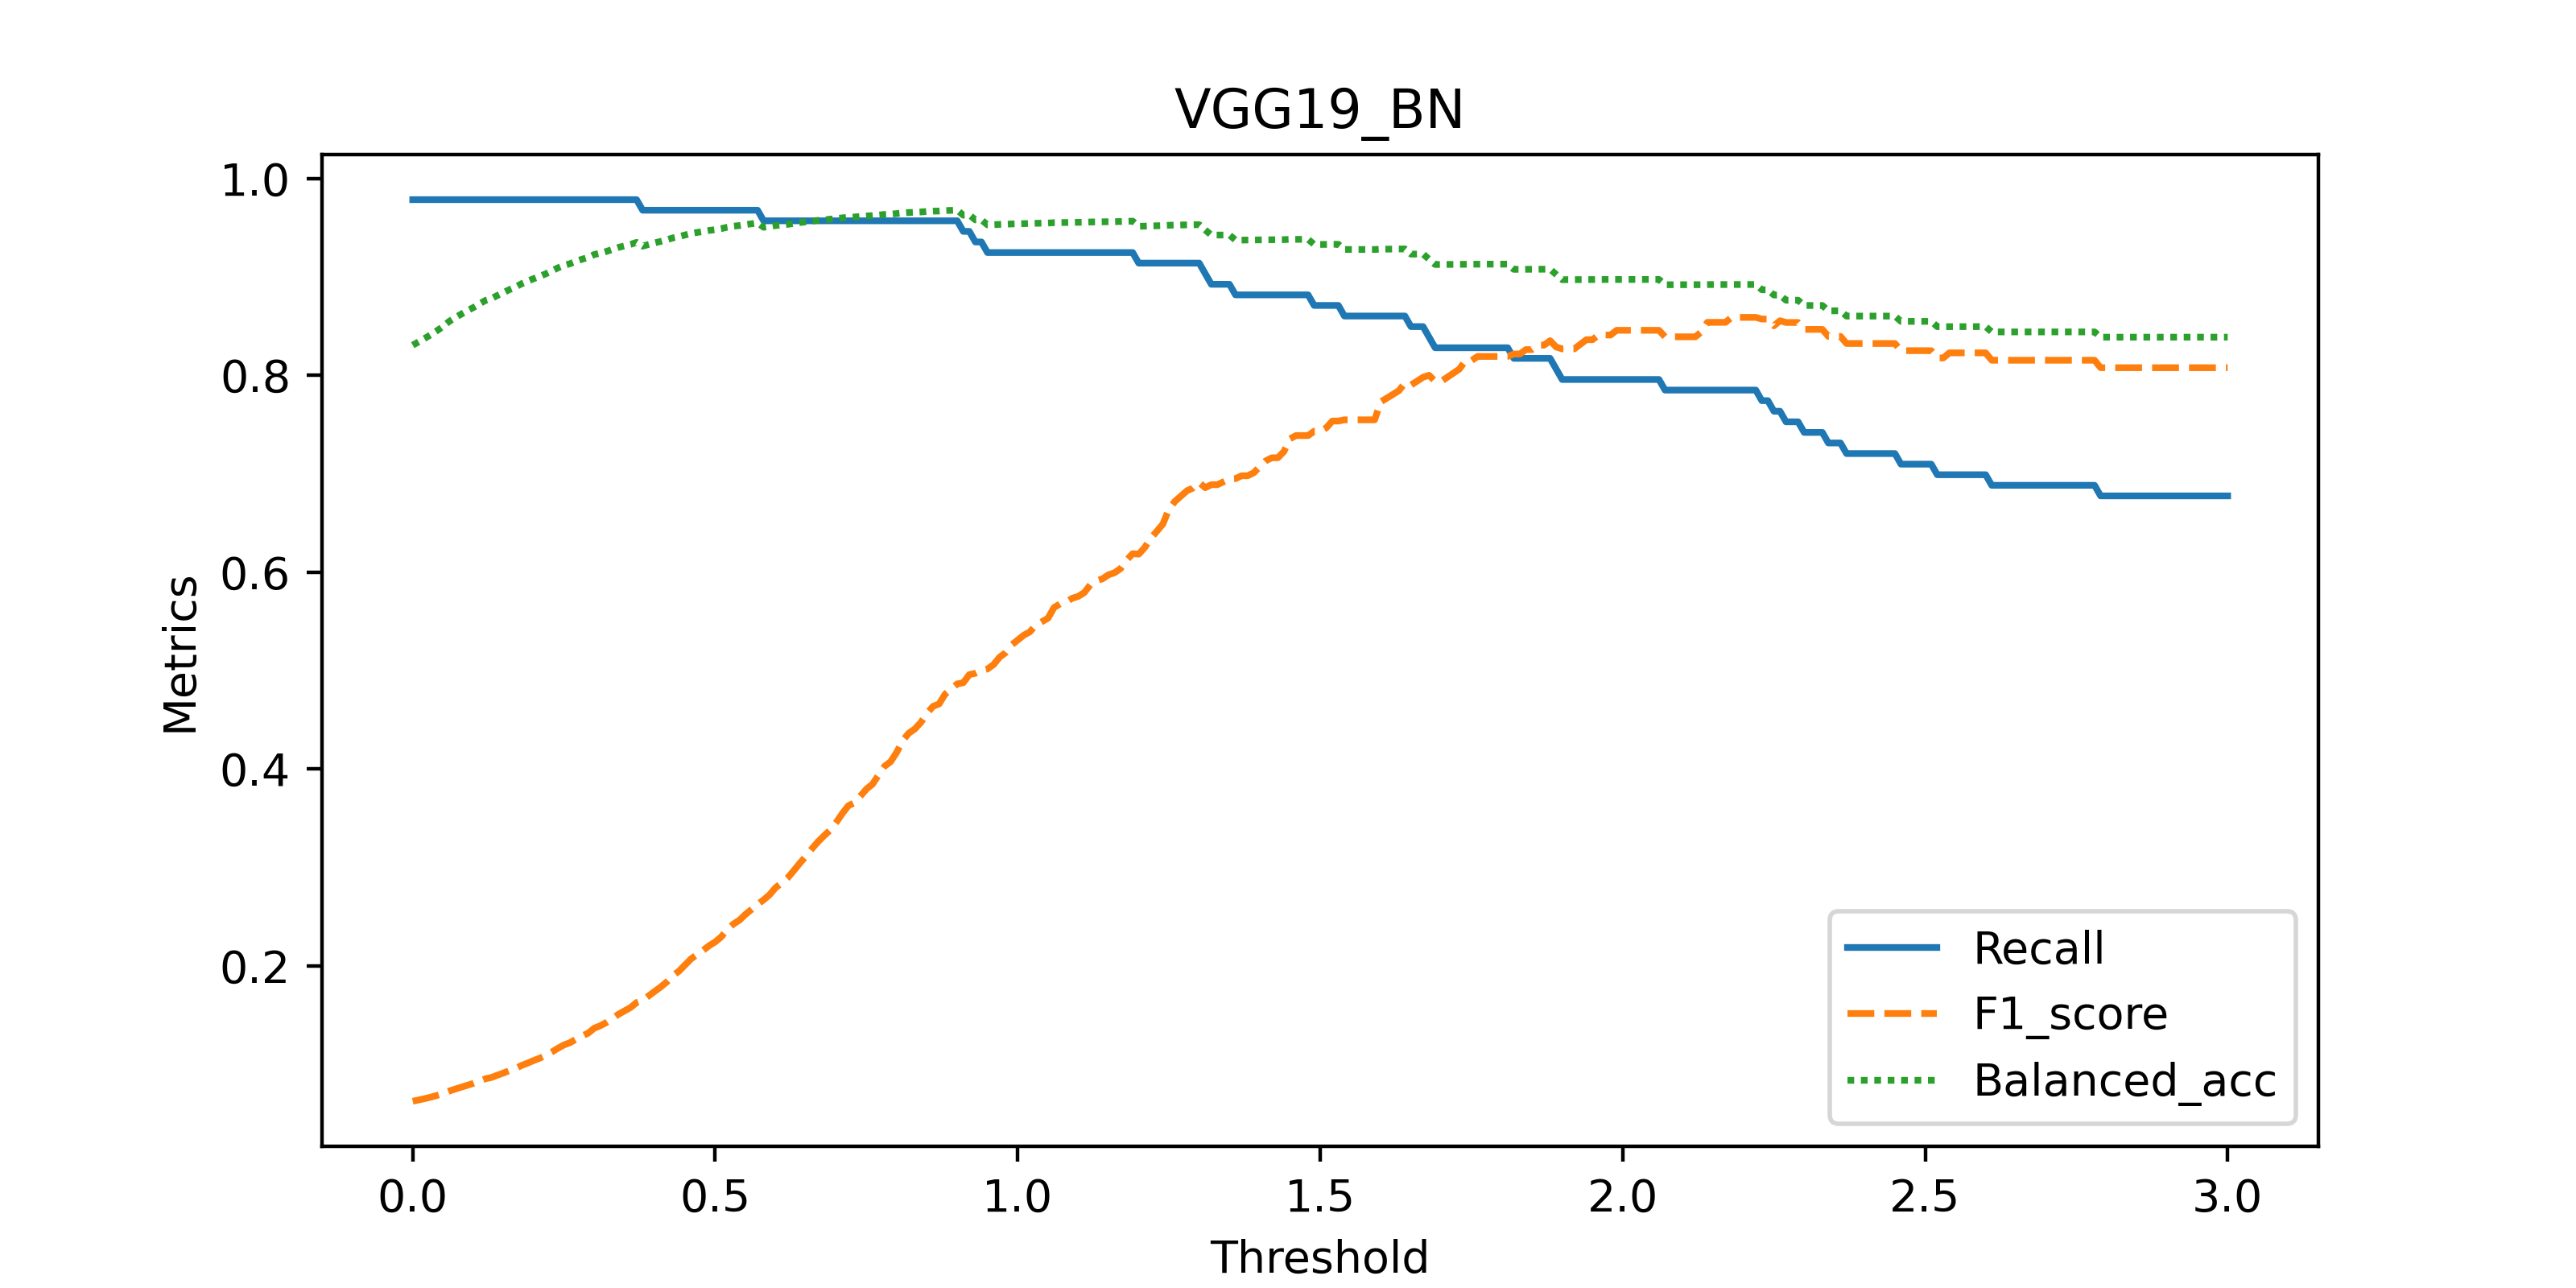
\includegraphics[width=\textwidth]{./results/comparison/VGG19_BN_threshold.png}
    \end{subfigure}
    \begin{subfigure}{0.48\textwidth}
        \centering
        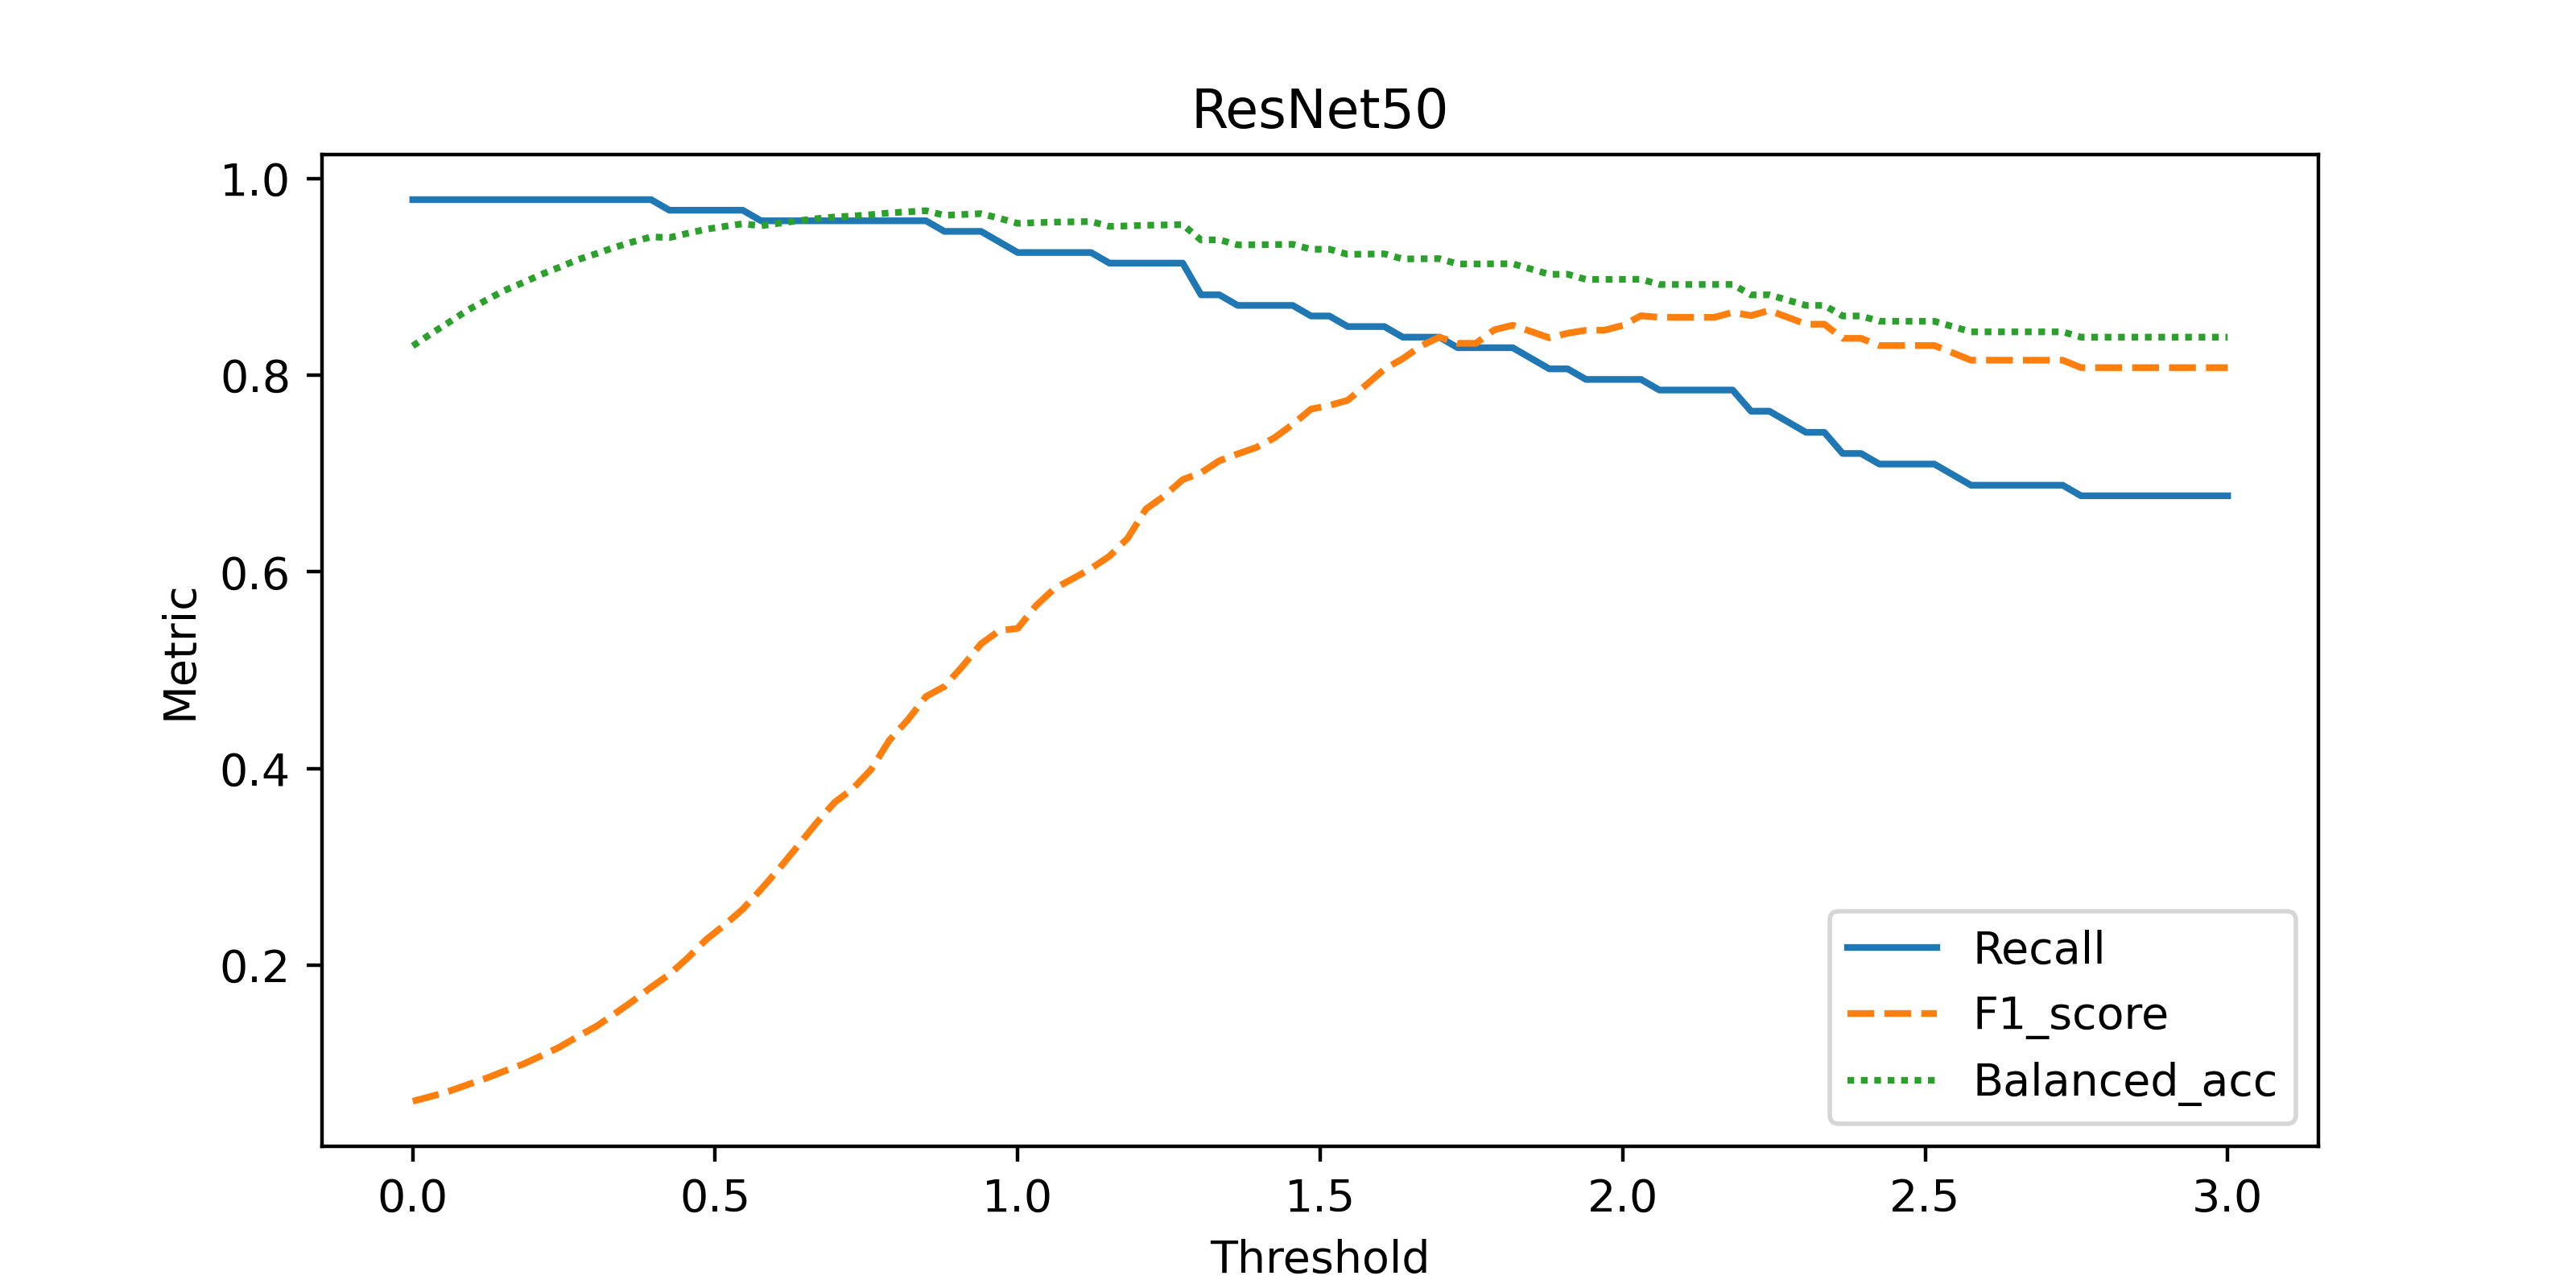
\includegraphics[width=\textwidth]{./results/comparison/ResNet50_threshold.png}
    \end{subfigure}
    \begin{subfigure}{0.48\textwidth}
        \centering
        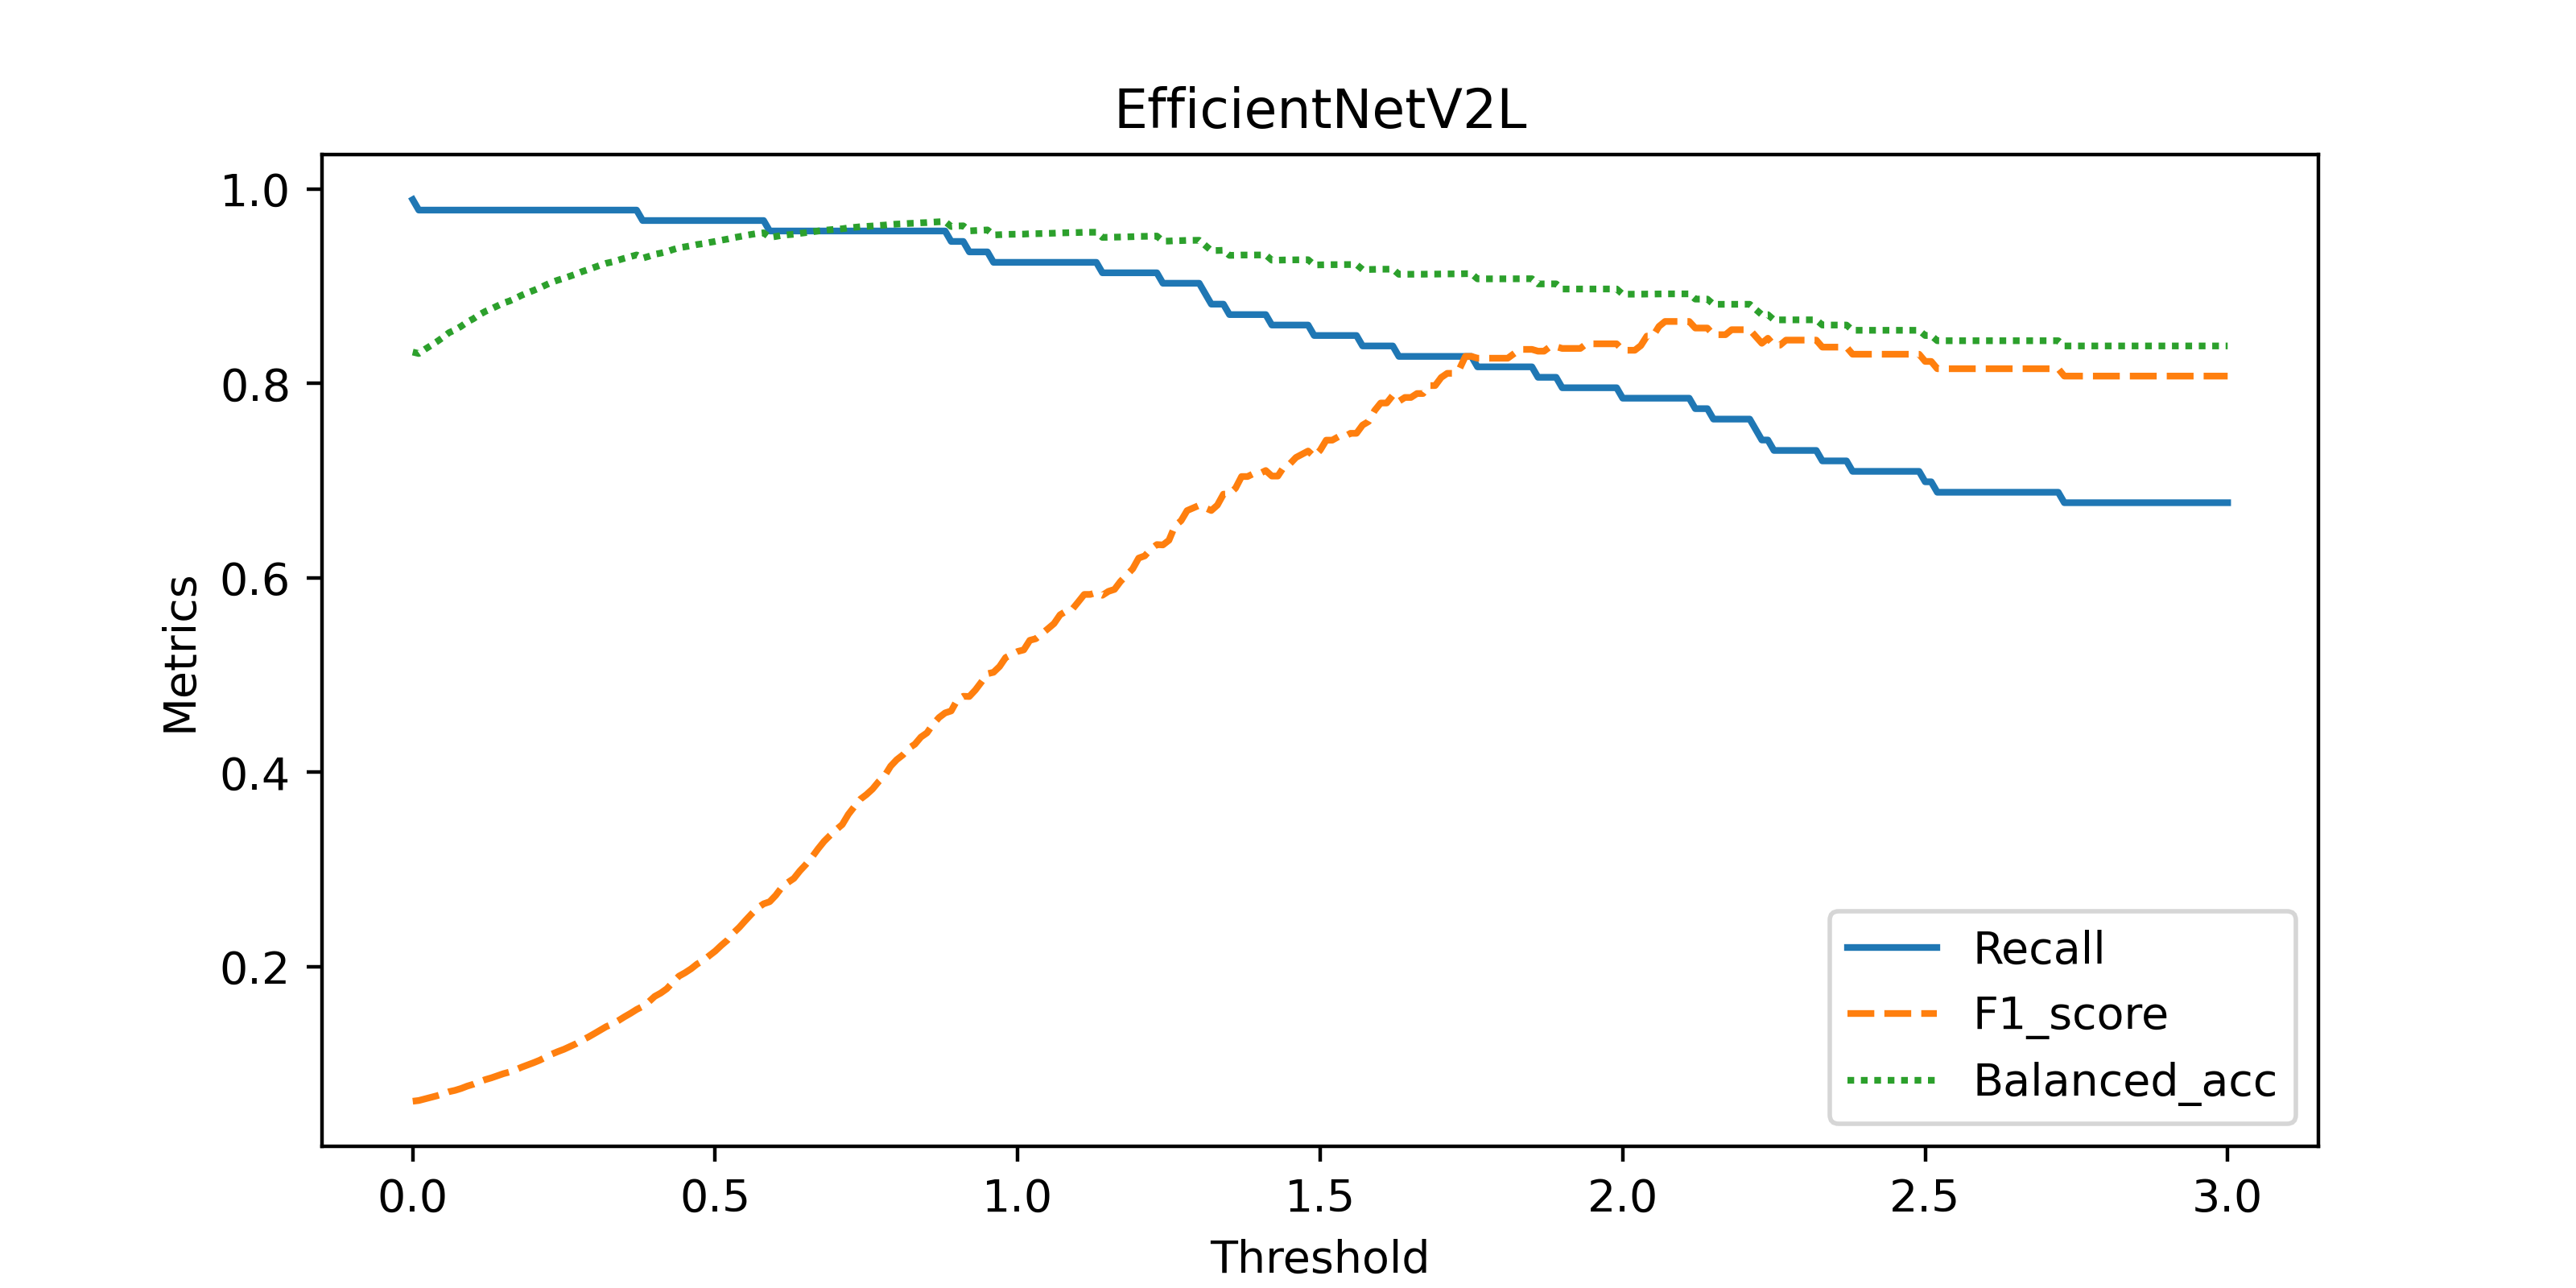
\includegraphics[width=\textwidth]{./results/comparison/EfficientNetV2L_threshold.png}
    \end{subfigure}
    \caption{Simulation of loss-based thresholds}
    \label{fig:threshold_simulation}
\end{figure}

\subsection{Detected anomalies}
To understand the learning capability of the Autoencoder, together with the anomaly detection
performance a visual analysis of the predicted or misclassified outliers is done.
The threshold for the loss-based approach was set to $2.15$ for all models.
A comparison of identified outliers is shown on Figure \ref{fig:outlier_comparison}.

\begin{figure}[H]
    \centering
    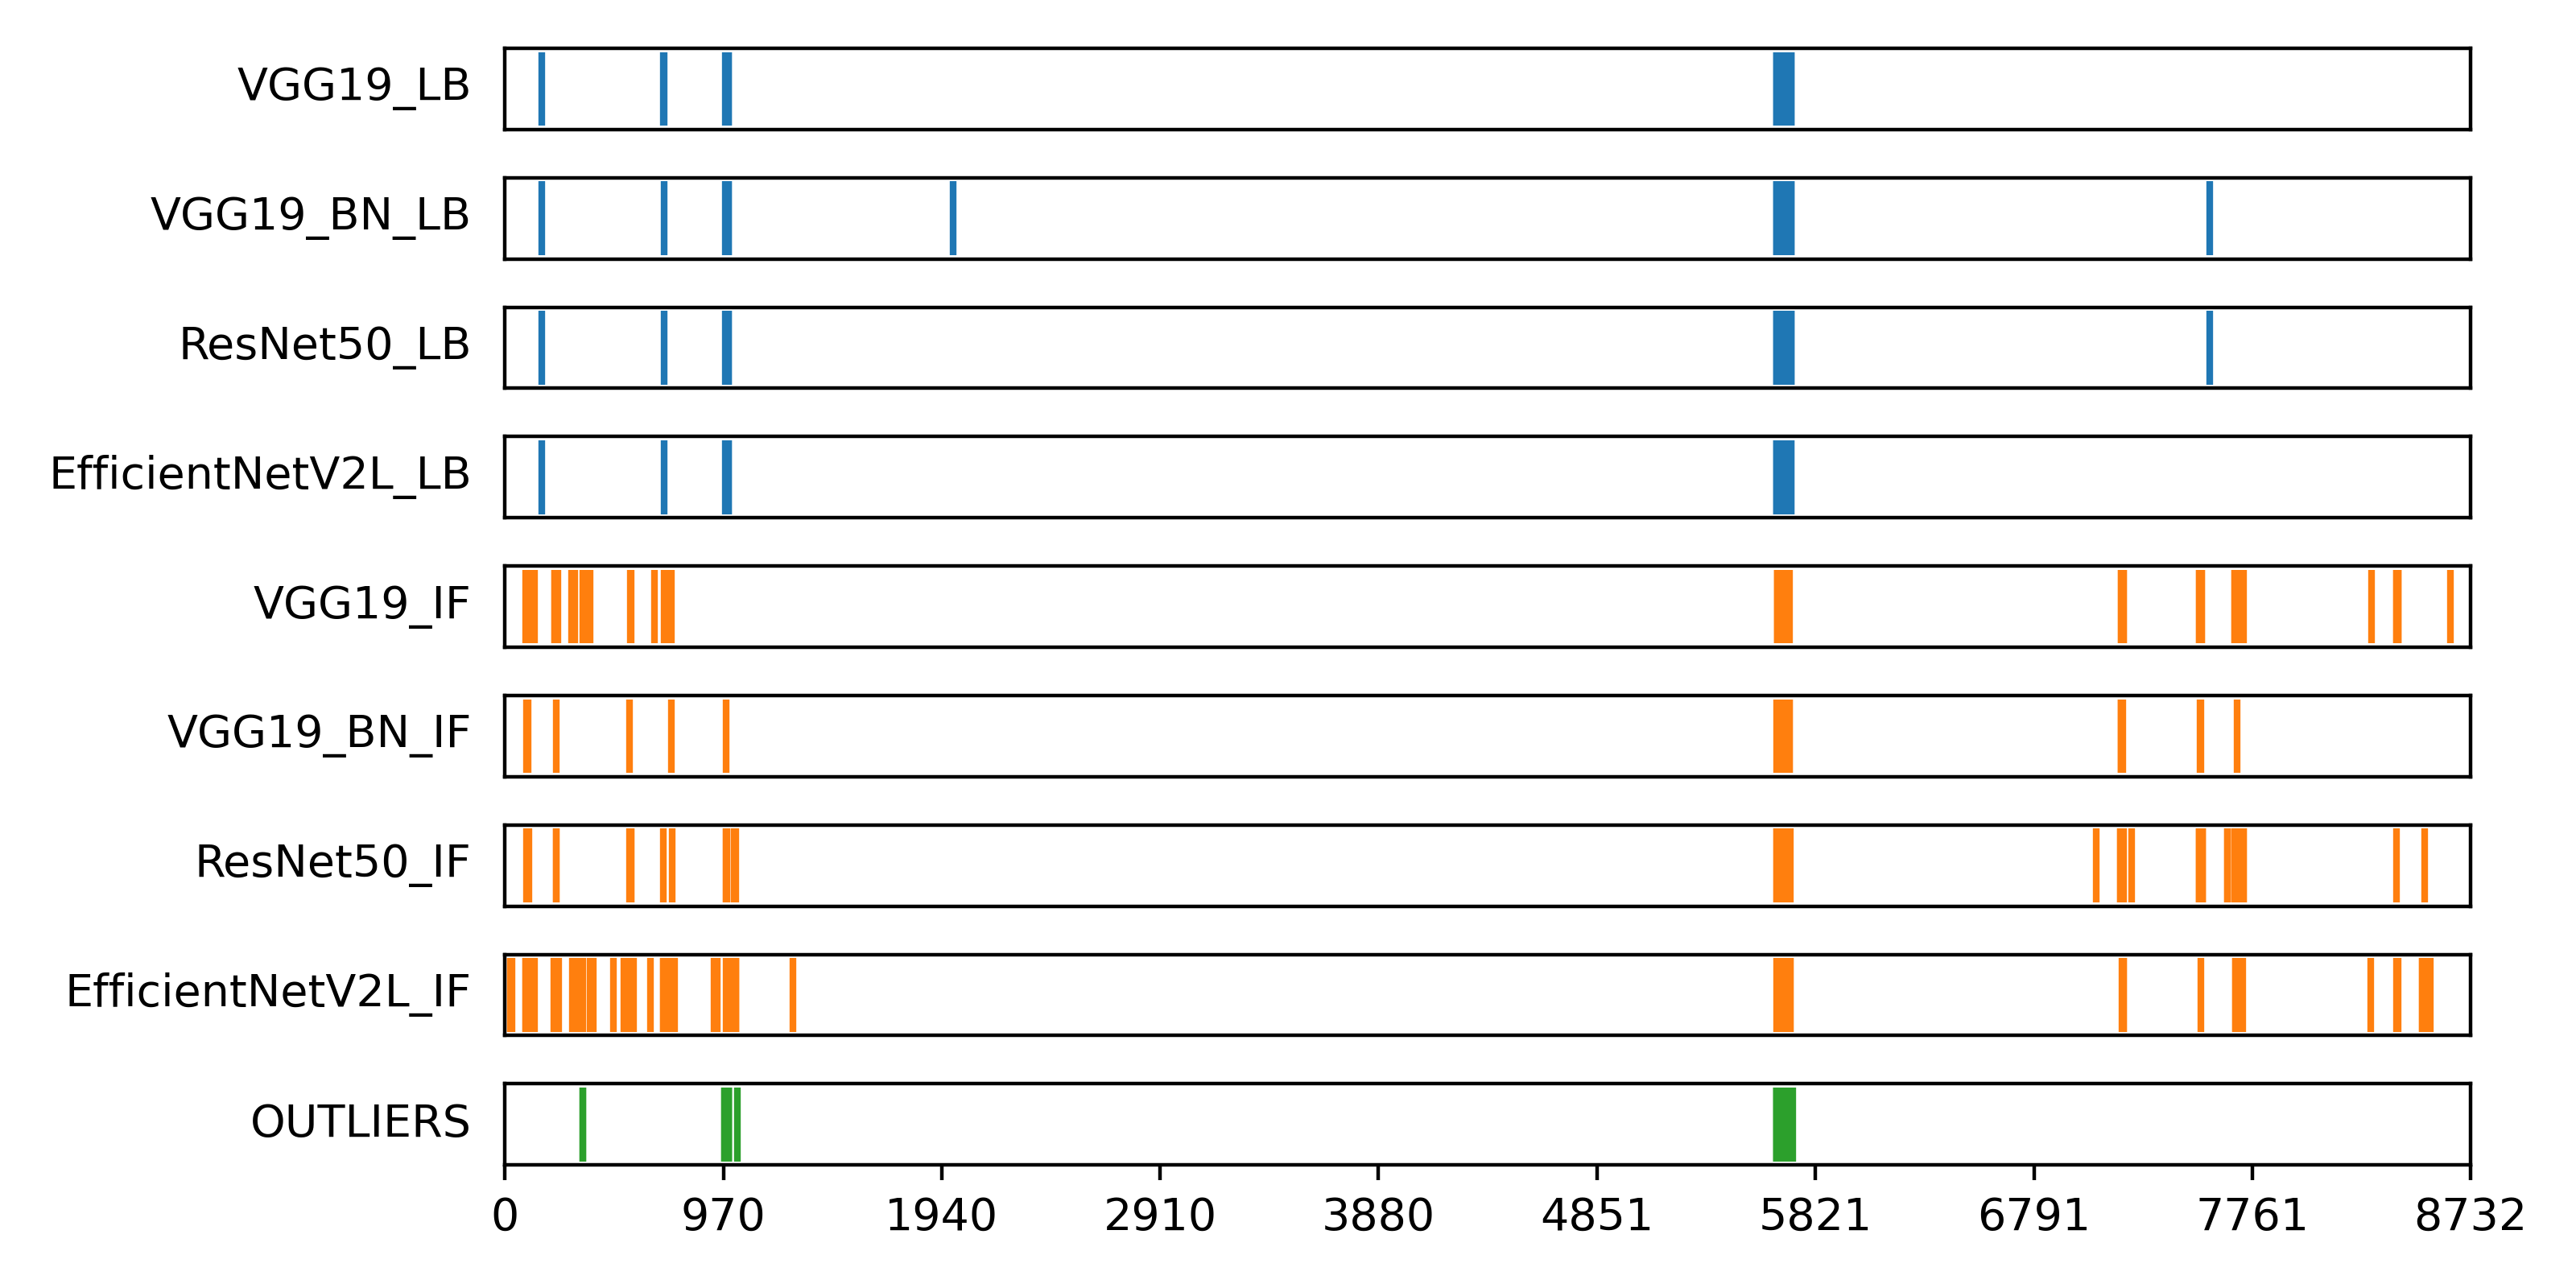
\includegraphics[width=\textwidth]{./results/comparison/outlier_comparison.png}
    \caption{Comparison of identified outliers of different models}
    \label{fig:outlier_comparison}
\end{figure}

The loss-based approach concentrates clearly on the clusters on the three main clusters of the
outliers, examples are shown on Figure \ref{fig:outlier_cluster_exampels}.
From a practical perspective, this already narrows down the search that has to be done on a full
video footage.
The Isolation Forest delivers also a good marking, almost all captures the three main clusters,
except the \emph{VGG19}, that misses the second cluster.
On the other hand, this approach delivers much higher rate of false positives.

\begin{figure}[H]
    \centering
    \begin{subfigure}{0.48\textwidth}
        \centering
        \includegraphics[width=\textwidth]{./data/sd1_sample/grass/img_00345.jpg}
        \caption*{Cluster 1}
    \end{subfigure}
    \begin{subfigure}{0.48\textwidth}
        \centering
        \includegraphics[width=\textwidth]{./data/sd1_sample/grass/img_00975.jpg}
        \caption*{Cluster 2}
    \end{subfigure}
    \begin{subfigure}{0.48\textwidth}
        \centering
        \includegraphics[width=\textwidth]{./data/sd1_sample/grass/img_05666.jpg}
        \caption*{Cluster 3}
    \end{subfigure}
    \begin{subfigure}{0.48\textwidth}
        \centering
        \includegraphics[width=\textwidth]{./data/sd1_sample/double_rail/img_05677.jpg}
        \caption*{Cluster 3}
    \end{subfigure}
    \caption{Examples of the three outlier clusters}
    \label{fig:outlier_cluster_exampels}
\end{figure}

From Figure \ref{fig:outlier_comparison} it can be seen that there are three false positive
indications resulting from almost all models at frame number $163$, $707$ and $7573$.
These are presented on Figure \ref{fig:false_positives}.
The samples indicate the presence of some grass or significant amount of ballast rocks
covering even the sleepers.
Deeper investigations on the reproduced output images reveal that the Autoencoder is
very sensitive to the presence of edges (please refer for example to Figure
\ref{fig:efficientnetv2l_examples}).
Such edges are resulting mostly from grass, therefore a small amount might be enough
to increase the probability of an outlier indication.
On the other hand, the lack of sleeper is removing some features from the decoded images,
providing a more homogeneous image, that might be misinterpreted by the anomaly detector.

\begin{figure}[H]
    \centering
    \begin{subfigure}{0.48\textwidth}
        \centering
        \includegraphics[width=\textwidth]{./data/sd1_sample/normal/img_00163.jpg}
        \caption*{Frame no. 163}
    \end{subfigure}
    \begin{subfigure}{0.48\textwidth}
        \centering
        \includegraphics[width=\textwidth]{./data/sd1_sample/normal/img_00707.jpg}
        \caption*{Frame no. 707}
    \end{subfigure}
    \begin{subfigure}{0.48\textwidth}
        \centering
        \includegraphics[width=\textwidth]{./data/sd1_sample/normal/img_07573.jpg}
        \caption*{Frame no. 7573}
    \end{subfigure}
    \caption{Remarkable false positives}
    \label{fig:false_positives}
\end{figure}